% ==================================================
% CHAPTER 4: Validating x-ray alignment parameters with cosmic muon data %
% ==================================================

\chapter{Validating x-ray alignment parameters with cosmic muon data}
\label{chap:comparison}
% Edit count: Lia - 0, Brigitte - 0

% --------------------------------------------------
\section{Presentation of theoretical method for comparison}
% --------------------------------------------------

The goal of this work is to validate the alignment parameters extracted from the x-ray data with cosmics data. The crux of the issue is that the x-ray dataset provides absolute local offsets while the cosmics dataset provides relative local offsets. The only solution is to analyze the x-ray data in the same relative coordinate system as cosmics.

The measured beam profile center provided by the x-ray data were affected by local offsets the same way as cosmics (equation \ref{eqn:local_translation}). Therefore, if a 2-layer track is abstracted from the beam profile center positions on each layer, and the residual calculated on a third layer, that residual should match the cosmics residual. For example, the position of the x-ray residuals calculated for the x-ray track on layer X calculated from the beam profile centers on layers Y and Z for QL2.P.11 is shown \textit{in the last chapter or in the figure below! Yet to decide. Ask Brigitte}. 

%\begin{figure}
%    \centering
%    
\includegraphics[width = \textwidth]{figures/potato.png}
%    \caption{Mean of residuals in each \SI{100}{\milli\meter} by \SI{100}{\milli\meter} bin over the area of the quad layer for QL2.P.11, with the position and value of the x-ray residuals plotted overtop.}
%    \label{fig:xray_beam_profile}
%\end{figure}

The track is "abstracted" because the beam profile center is actually the Gaussian mean of all selected cluster centroids that were recorded during the x-ray data taking period. This was the best analysis method because since the x-rays cause signal in the chamber via the photoeffect, there were not individual "x-ray tracks" to record. In fact the x-ray data was collected separately for each layer. However, since the effect of local offsets on the so-called x-ray residuals would be the same, the difference in algorithm between x-ray and cosmics analysis did not matter. 
ROUGH

The uncertainty in the individual x-ray residuals depending on the tracking combination, however
Note that the mean of cosmics residuals around the x-ray points were calculated in bins exactly centered on the nominal x-ray gun position. The area of the region of interest in which to include cosmics tracks to calculate the mean of cosmics residuals was chosen by . . . 

Every possible tracking combination was used to get enough x-ray residuals to see the correlation, which is clear in figure~\ref{fig:correlation}.

\begin{figure}
    \centering
    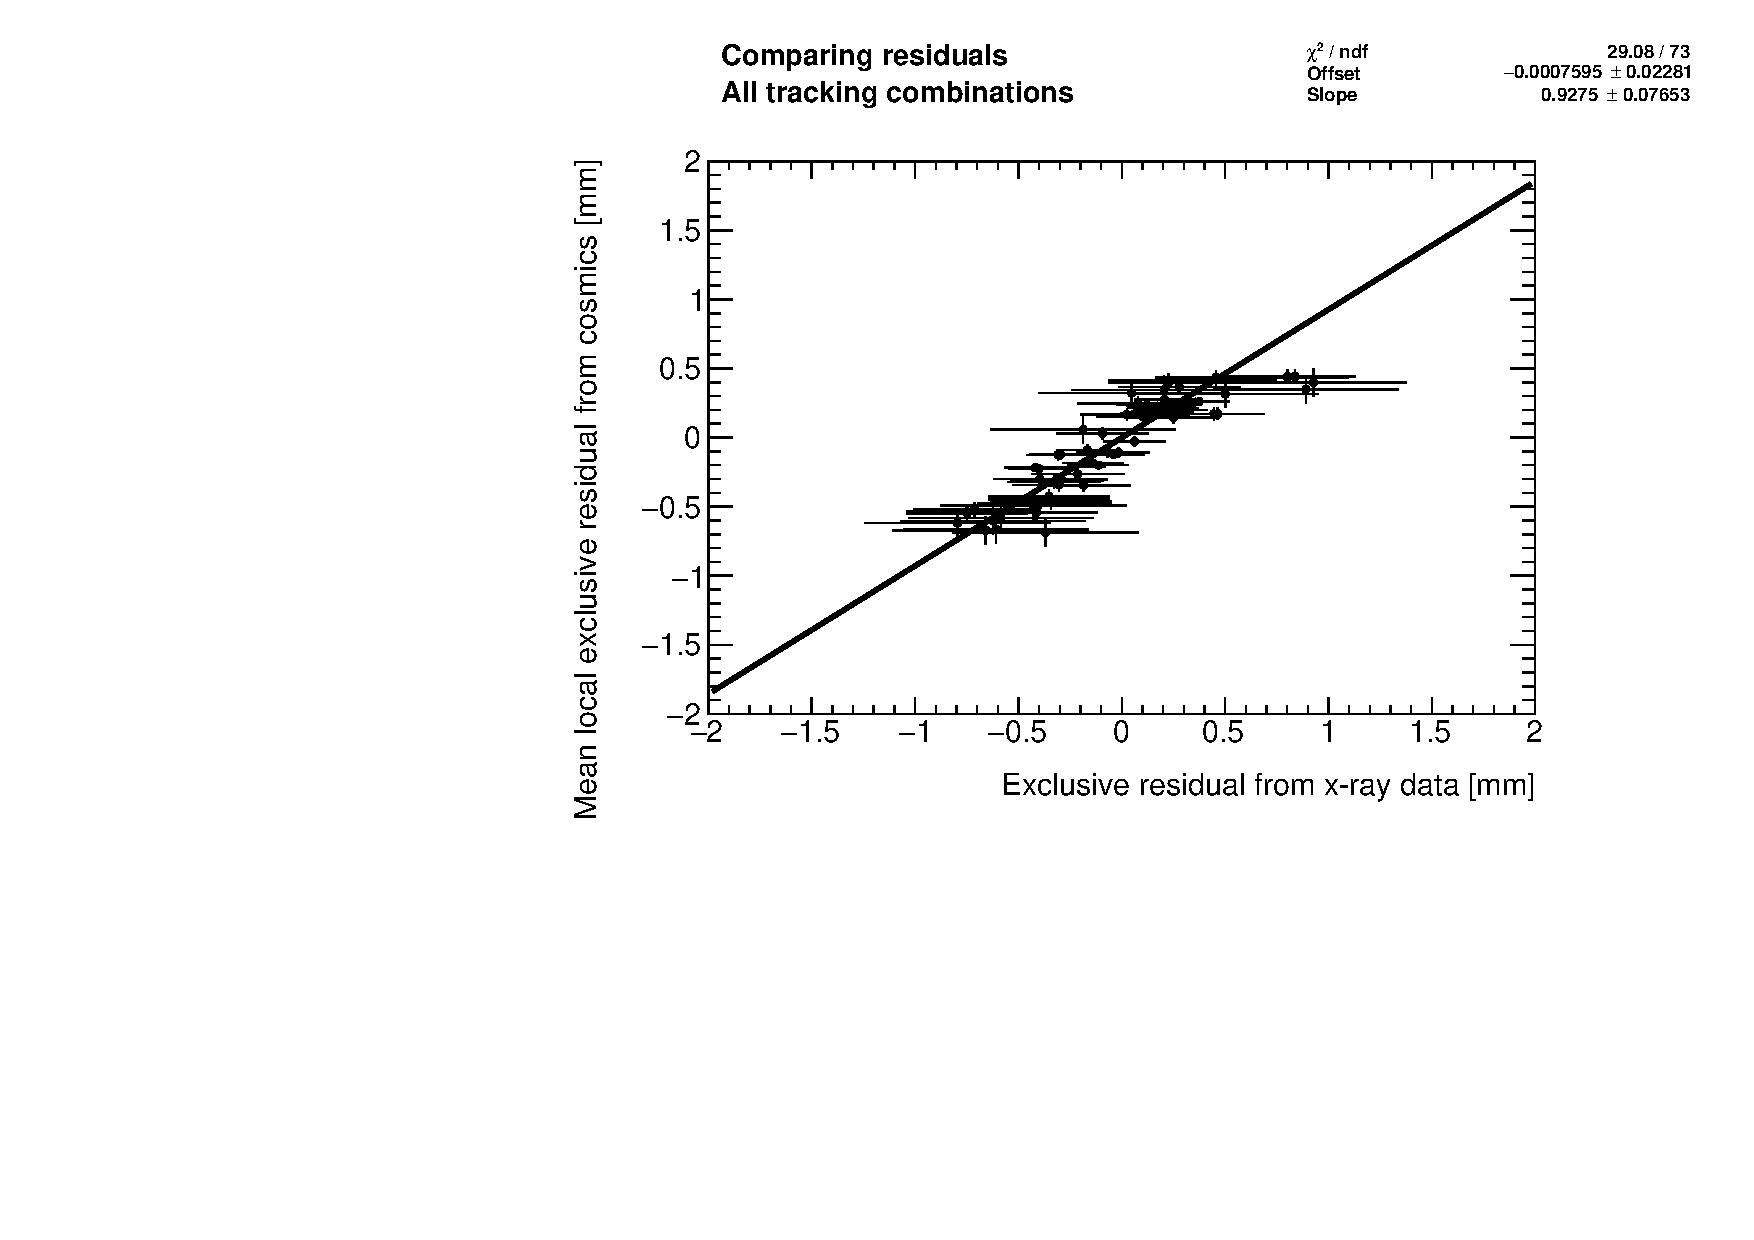
\includegraphics[width = \textwidth]{figures/QL2P11_3100V_2021-08-05_local_mean_cosmics_residual_vs_xray_residual_scatter_all.pdf}
    \caption{Correlation plot between x-ray and cosmics residuals for all tracking combinations for QL2.P.11. }
    \label{fig:correlation}
\end{figure}

First, the fitted slope and offset in figure~\ref{fig:correlation} show that the two datasets largely support one another for QL2.P.11. After testing a few quadruplets of each geometry built in Canada, the conclusion was the same. However, the magnitude of the uncertainties in the x-ray residuals

To say:
- Interps have smaller errors and typically smaller values than extraps
- Uncertainties set the scale on which we are sensitive
- Cosmics has smaller uncertainties => potential to constrain misalignment model with cosmics data.

% Comparing x-ray and cosmics residuals is precisely what was done with the new software package \package{strip_position_analysis}. Several quadruplets of each Canadian geometry were tested using this method, and every possible tracking combination was used to get enough comparison points to check the correlation. 

%TODO : include that x-ray data is collected layer by layer

% --------------------------------------------------
\section{Limitations}
% --------------------------------------------------
An x-ray gun position was only useful if data was recorded on at least 3 layers to be able to calculate a residual. As a result, the number of x-ray residuals for QL2s is around 70 while it is much smaller for QS3Ps.

